\section{Unsupervised Routine discovery}
%02 12 2014
Topic models are algorithms for discovering the main themes that pervade a large and otherwise unstructured collection of documents. Data are treated as observations arising from a generative probabilistic process in which hidden variables reflect the thematic structure of a collection of documents. The intuition behind the use of the Latent Dirichelet Allocation (LDA) to discover PA routines is that each day is a mixture of thematically coherent PA measures as a text document is a mixture of thematically coherent terms. The graphical model for LDA is provided in Fig.~\ref{fig:LDA_model}.
%%%%%%%%%%%%%%%%%%%%%%%%%%%%	FIGURE TOPICMODEL		%%%%%%%%%%%%%%%%%%%%%%%%%%%%
\begin{figure}[ht]
\centering
    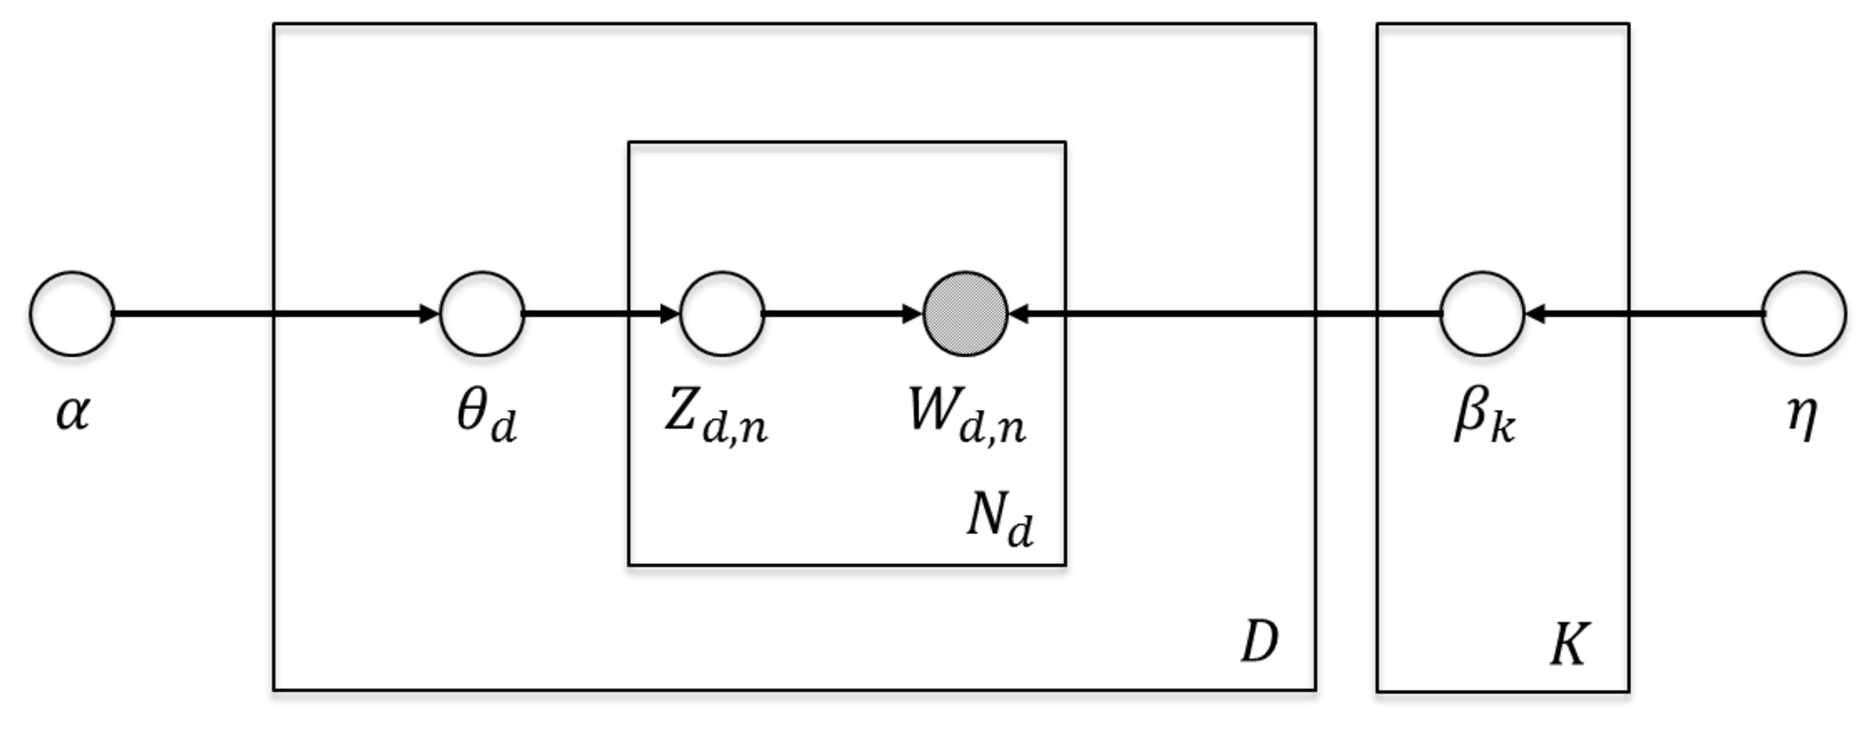
\includegraphics[width=.40\textwidth]{figure/eps/LDA_model.eps}
  \caption{Graphical model for LDA. Each node is a random variables, edges denote possible dependences. The only observed variables are the words (shaded).}\label{fig:LDA_model}
\end{figure}
%%%%%%%%%%%%%%%%%%%%%%%%%%%%%%%%%%%%%%%%%%%%%%%%%%%%%%%%%%%%%%%%%%%%%%%%%%%
All the assessed days (also called documents $d_{1:D}$) share the same set of daily routines (also called topics $\beta_{1:K}$) that are defined as Dirichelet distributions over the observed set of PA descriptors (also called words $W$ of a fixed vocabulary). Observing activities in patients is a difficult task since it is time-intensive and intrusive. At the same time patients are not able to accurately self-report their physical activities~\cite{Pitta_2007} and the training of a classifier requires annotations that in a daily life scenario are difficult to obtain. In order to make the methodology fully unsupervised we assume that the observed words (input of the model) are composed by multimodal PA measures coming from a body area sensor network.
Each assessed day exhibits PA daily routines in different proportion indicated as $\theta_{1:D}$, i.e. each day has a different distribution over the routines that also follow a Dirichelet distribution. The distribution of the words in a routine and the distribution of the routine in a document depend only on the topic hyper-parameters $\eta$ and $\alpha$ that control the mean shape and sparsity of the distributions. In such a model the $N$ words ($W_{d,n_{1:N}}$) that compose the $D$ documents are the only random variables observed and depend on the per word topic assignment ($Z_{d,n}$) and all the $\beta_{k}$.
The daily routines then are composed indirectly by low-level PA measures that belong, with a certain probability distribution, to different thematic areas. Different routines will have different PA measures with different probabilities. The generative process of the model defines a joint probability distribution over both the observed and hidden random variables, according to:
\begin{dmath*}
  p(\beta_{1:K},\theta_{1:D},Z_{1:D},W_{1:D}) = \prod_{k=1}^{K} p(\beta_{k}|\eta) \prod_{d=1}^{D} p(\theta_{d}|\alpha) \prod_{n=1}^{N} p(Z_{d,n}|\theta_{d}) p(W_{d,n}|Z_{d,n},\beta_{1:K}).
\nonumber\end{dmath*}
Reversing the generative process, it is possible to calculate the hidden structure that likely generated the observed collection of document. More formally the joint probability distribution is used to compute the conditional distribution of the hidden variables given the observed variables by: 
\begin{dmath}
  p(\beta_{1:K},\theta_{1:D},Z_{1:D}|W_{1:D}) =   \frac{p(\beta_{1:K},\theta_{1:D},Z_{1:D},W_{1:D})}{p(W_{1:D})}.
  \label{eq:conddistr}
\end{dmath}
This conditional distribution is also called the posterior distribution and it is intractable to compute. Topic modelling algorithms compute an approximation of~(\ref{eq:conddistr}) by finding a distribution over the latent topic structure to be close to the true posterior. In particular, for this analysis, we use variational inference that posits a parameterized family of distributions over the hidden structure and then finds the member of that family that is closest to the posterior according to \emph{Kullback-Leibler} divergence.

%put in the claims
%In the implementation described in the follwing paragraph we propose a methodology to create a vocabulary of meaningful words from a set of mutimodal PA measures, we discover PA routines that pervade daily life of COPD patients. Finally, we infer the underlying topic structure of numerous patients data. In particular, for each assessed day we infer which is the distribution over the routines found and we describe the temporal regularities of the multidimensional constructs and parameter of PA.




%LDA falls precisely into this framework.
%The observed variables are the words of the documents; the hidden variables are the topic structure; and the generative process is as described here. The computational problem of inferring the hidden topic structure from the documents is the problem of computing the posterior distribution, the conditional distribution of the hidden variables given the documents.
%We can describe LDA more formally with the following notation. The topics
%are b1:K, where each bk is a distribution over the vocabulary. The topic proportions for the dth document are qd, where qd,k is the topic proportion for topic k in document d (the cartoon histogram in Figure 1). The topic assignments for the dth document are zd, where zd,n is the topic assignment for the nth word in document d (the colored coin in Figure 1). Finally, the observed words for document d are wd, where wd,n is the nth word in document d, which is an element from the fixed vocabulary.
